\section{Upgrade of the CMS tracker system}

\graphicspath{{5_Outlook/Figures}}

The Large Hadron Collider (LHC) will be upgraded to the High-Luminosity LHC (HL-LHC) configuration. Currently,
this upgrade is planned to take place in Long-Shutdown-3 era between 2026 and 2029, and HL-LHC is expected to 
start running starting from 2029.
With HL-LHC, the instantaneous luminosity is expected to reach an unprecedented peak of
$7.5 \times 10^{34}$ \lumiunit, with an average number of pileup interactions up to $200$. To cope with
the increased instantaneous luminosity, the CMS detector will be upgraded, which is known as the Phase-2 upgrade.
One crucial upgrade will be in the tracker detector, which is the closest detector to the proton-proton collision point. 
Hence, to cope with the demanding operating conditions, the CMS tracker detector will be replaced. The aim of the
new tracker detector is to provide robust tracking under increased instantaneous luminosity, and also provide inputs
to the Level-1 (L1) trigger~\cite{CMS:Phase2TrackerUpgrade}, which is also a crucial physics goal since having tracking
information at L1 trigger will improve the data selection performance.

The Phase-2 tracker of CMS will be composed of two parts:
Inner tracker (IT) and outer tracker (OT), as shown in Fig.~\ref{fig:phase2_tracker_layout}. 
The IT is made of silicon
pixel detectors, and OT is made of silicon micro-strips and macro-pixel detectors.
Both IT and OT are designed to have better radiation hardness and higher
granularity compared to the current tracker detector. Furthermore, the tracking acceptance will be extended
in the forward region, with the IT covering a range up to $|\eta| < 4$, as can be seen in 
Fig.~\ref{fig:phase2_tracker_layout}.

\begin{figure}[htbp]
    \centering
    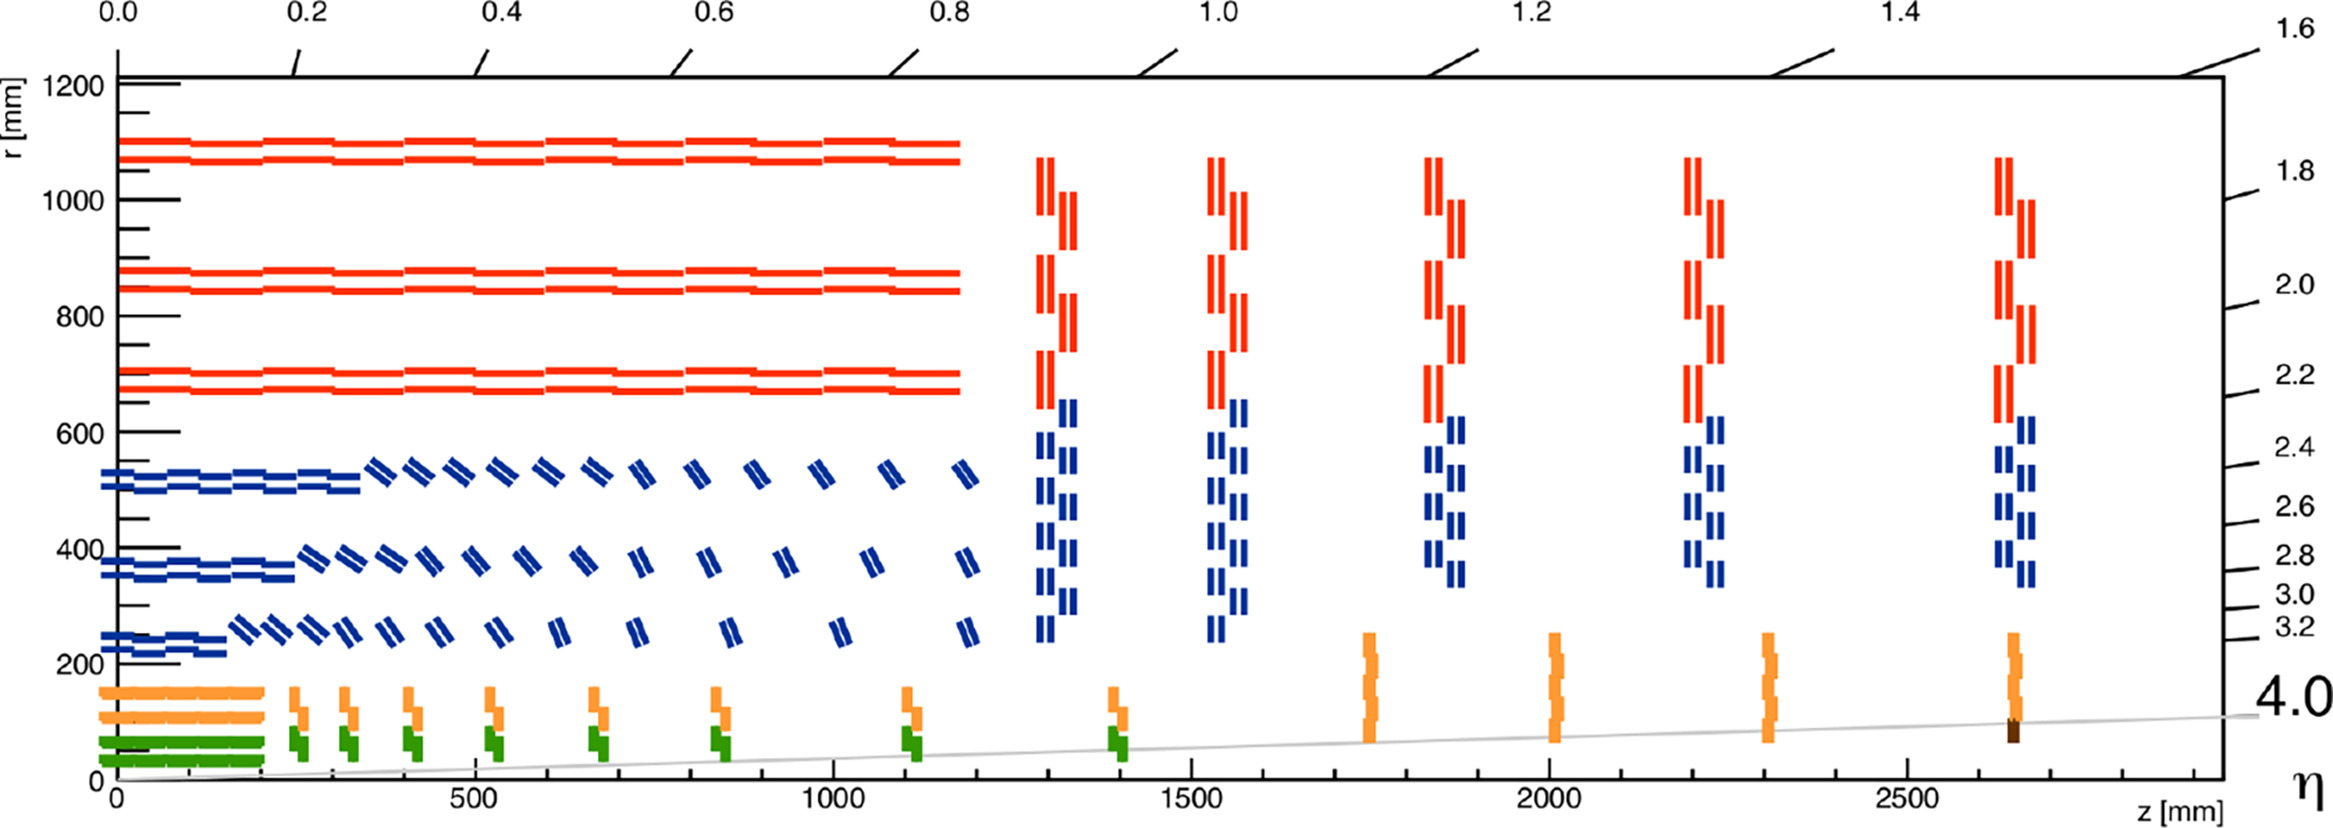
\includegraphics[width=0.9\textwidth]{TrackerUpgrade/phase2_tracker_layout.jpeg}
    \caption{Layout of the CMS Phase2 tracker detector, each colored line indicates a detector module. 
    Pixel modules, in orange (quad-chip modules) and green (double-chip modules), form the inner tracker system. 
    The outer tracker is composed of two different types of modules indicated with blue (PS modules) and red (2S modules) lines. 
    One quarter of the detector is shown. Figure taken from~\cite{CMS:Phase2TrackerUpgrade}.}
    \label{fig:phase2_tracker_layout}
\end{figure}

The IT will cover a total area of $4.9$ \msq with 3892 silicon modules. There will be two types of silicon modules deployed:
Double-chip (1x2) modules and quad-chip (2x2) modules. The arrangement of modules in the detector is shown in Fig.~\ref{fig:phase2_tracker_layout},
where double-chip modules are denoted with green, and quad-chip modules are denoted with orange. A detailed overview of
IT and OT features and the upgrade planning is given in \cite{CMS:Phase2TrackerUpgrade}.

The OT consists of dual-sensor modules, sometimes also called ``$\pt$-modules'', which are two closely spaced silicon
sensors read out by the same electronics. A charged particle traversing the module will leave a signal in both sensors,
and readout electronics can compare the two hit positions. Once the hit position in the first sensor is identified,
the hit position in the second sensor will depend on the track curvature in the magnetic field, which is then related
to the $\pt$ of the charged particle. If the hit in the second sensor is within the correlation window relative to the
hit in the first sensor, a track segment (called stub) is generated and the tracks will be reconstructed. It should be
noted that this procedure is equivalent to the requirement of a minimum $\pt$ of the charged particle, since the particles with
lower $\pt$ will experience more bending, and are more likely to fall out of the correlation window. The $\pt$ threshold is
set by the spacing between the two sensors in the module, and can be tuned in order to have a threshold of between $2$ and $3$
GeV~\cite{CMS:Phase2TrackerUpgrade}. A schematic of such dual-sensors is shown in Fig.~\ref{fig:stub_ot_schematic}.

\begin{figure}[htbp]
    \centering
    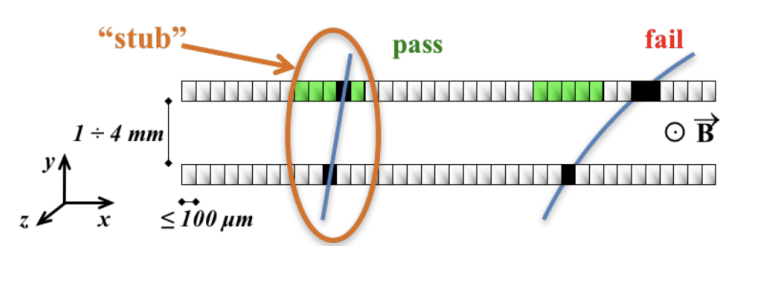
\includegraphics[width=0.8\textwidth]{TrackerUpgrade/stub_ot_schematic.png}
    \caption{Schematic showing the functioning of dual-sensor OT modules. The high-$\pt$ track on the left
    experiences smaller bending due to the magnetic field and falls into the green correlation window, thus producing
    a stub. The low-$\pt$ track on the right however, experiences larger bending and falls out of the correlation
    window, and does not generate a stub. Figure taken from~\cite{CMS:TrackerUpgradeStatus}.}
    \label{fig:stub_ot_schematic}
\end{figure}

All silicon modules, both in the IT and OT, communicate with CMS back-end data acquision system (DAQ) 
optically through low power GigaBit transciever (lpGBT) links, which run at speeds of 5-10 Gbps
in uplink mode (\textit{i.e.,} from front-end electronics to DAQ), and 2.56 Gbps in downlink mode~\cite{CMS:TrackerUpgradeStatus}. 
In the service cavern, sets of Data Trigger and Control (DTC) cards are placed 
at the receiving end of the lpGBT optical links
coming from the IT and OT modules. The DTCs are high bandwidth processors based on commercial FPGAs. Their task
is to receive data from the IT and OT modules, which represent the hits pertaining to the triggered events, and
forward them to the DAQ system. The schematic of this workflow is shown in Fig.~\ref{fig:daq_schematic}.

\begin{figure}[htbp]
    \centering
    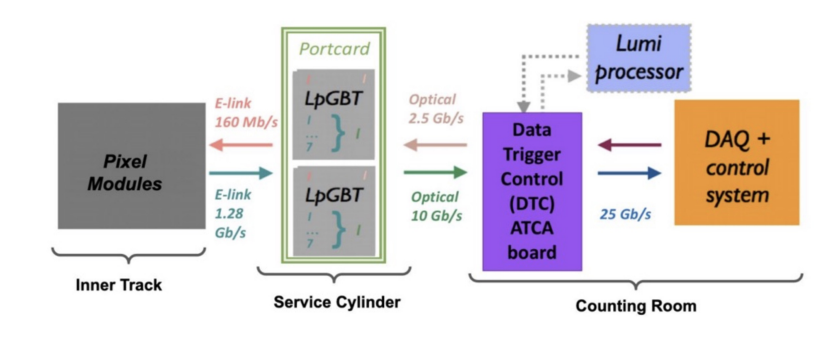
\includegraphics[width=0.8\textwidth]{TrackerUpgrade/daq_schematic.png}
    \caption{Schematic representation of the data acquisition system (DAQ) for the CMS Phase2 tracker.
    Figure is taken from~\cite{CMS:Phase2TrackerUpgrade}.}
    \label{fig:daq_schematic}
\end{figure}

In the case of OT, the DTC boards are also tasked with forwarding hit information in the detector to the Track
Finder Processors (TFP). When track segments (stubs) are generated from the dual-sensors in the OT, 
DTCs are tasked with forwarding the stub coordinates to TFPs, after converting the coordinates 
to the global reference frame~\cite{CMS:TrackerUpgradeStatus}. 

The Apollo board is used for the IT DTC, and is designed and developed at Boston University~\cite{CMS:ApolloPaper}.
In order to meet the design
criteria with high processing and bandwidth requirements, the Apollo uses high performance Xilinx Ultrascale+ Virtex
FPGAs, and 12-channel, 25 Gbps-per-channel optical transcievers to implement their functions~\cite{CMS:TrackerUpgradeStatus}.
The board is designed to comply with the Advanced Telecommunications Computing Architecture (ATCA) design 
specifications~\cite{PICMG:ATCA}.
The following subsection goes into more detail about the Apollo board architecture and the hardware components.

\subsection{Apollo DTC Board: The Design}

The Apollo DTC board is designed to provide a reusable hardware interface for different types of applications within the
CMS (and ATLAS) detector. It is composed of two main modules: A service module (SM) and a command module (CM).
The Apollo SM is an ATCA-compliant front board which provides power, communications and control infrastructure.
On the other hand, Apollo CM is a module with two Xilinx Ultrascale+ Virtex FPGAs, which can be programmed with
application specific firmware, hence making the Apollo hardware reusable across different applications. 

The CM is connected to the SM using 2 board-to-board connectors, which provide electrical and mechanical 
connectivity between the SM and CM. Apollo SM provides multiple interfaces to communicate with the CM,
providing I2C, UART, JTAG and AXI chip-to-chip links to the CM.
A block diagram of Apollo SM and CM is shown in Fig.~\ref{fig:apollo_schematic} (left), together with
a schematic of the Apollo SM (right).

\begin{figure}[htbp]
    \centering
    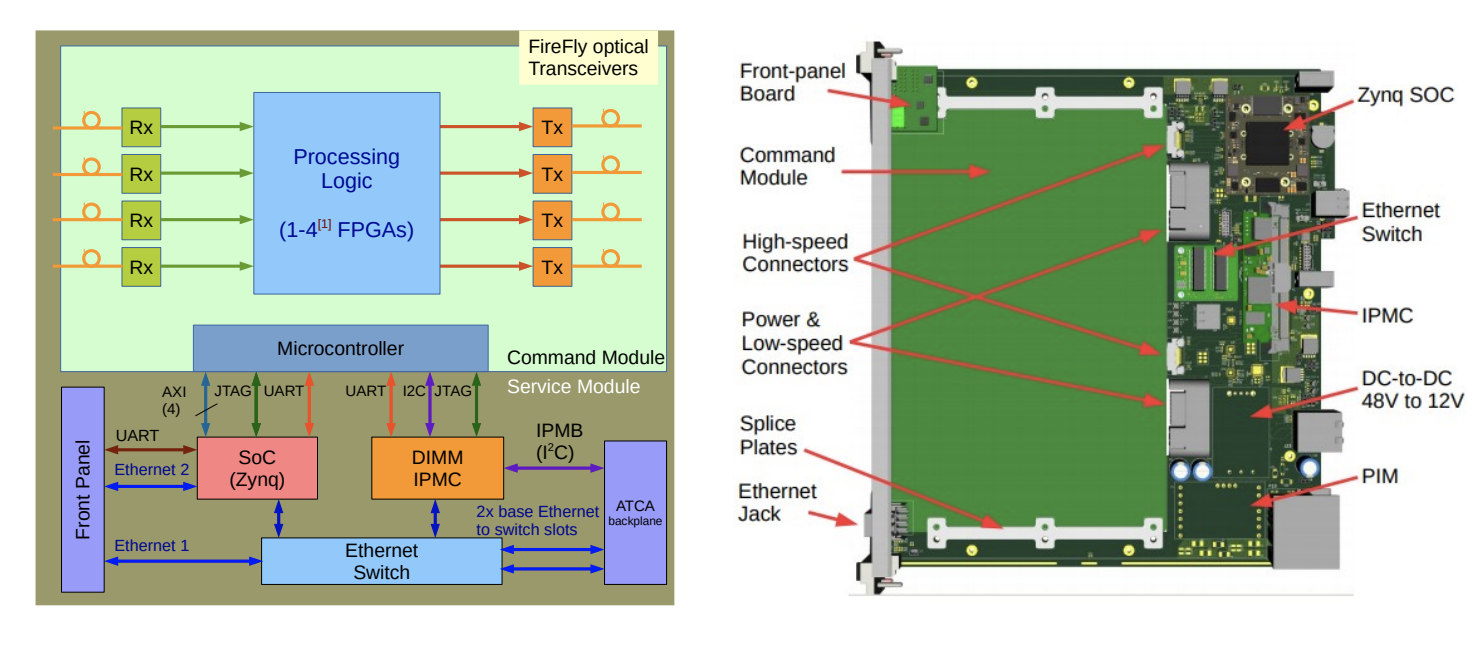
\includegraphics[width=0.95\textwidth]{TrackerUpgrade/Apollo/apollo_schematic.png}
    \caption{Block diagram of Apollo SM and CM (left) and a schematic of the Apollo SM (right). The SM provides
    multiple connection interfaces to the CM (I2C, AXI chip-to-chip, JTAG, UART), and the CM includes FPGAs with
    application specific firmware. Each SM is connected to a front-end panel as specified by the ATCA standards. 
    Schematics are taken from~\cite{CMS:ApolloPaper}.}
    \label{fig:apollo_schematic}
\end{figure}

\subsubsection{Apollo Service Module}

The Apollo SM hosts a Xilinx Zynq Ultrascale+ system-on-chip (SoC),
which provides a 64-bit ARM processor core, together with an FPGA and memory interfaces. A userspace I/O (UIO) driver
is used to map the register addresses from different devices on the SM and CM, to the memory space of the Zynq SoC.
This way, also using the AXI chip-to-chip interface to the CM, monitoring data from registers on the CM 
can be read out, including current and temperature values in the CM. The SoC also provides a JTAG interface to the CM,
which makes it possible to program the FPGAs located in the CM through the SoC on the SM.

Another important component of the SM is the Intelligent Platform Management Controller (IPMC), also specified
within the ATCA design standards. The essential functions of the IPMC can be summarized as follows:

\begin{itemize}
    \item Manage the power up and power down sequences of the Apollo board.
    \item Provide communication with the ATCA shelf manager by reading a set of monitoring values 
    (temperature, current and voltage) from on-board sensors and deliver them to the shelf manager.
\end{itemize}

For the Apollo SM, the OpenIPMC hardware is used~\cite{Calligaris:OpenIPMC}. OpenIPMC is a
Cortex-M7 ARM-core based microcontroller, which provides flash memory and multiple I/O peripheral interfaces
to communicate with the other devices on Apollo SM and CM. OpenIPMC firmware is written in C language, and it is 
based on the FreeRTOS real-time operating system, allowing the microcontroller to process multiple tasks
in parallel using the FreeRTOS scheduler. Most of these tasks are a part of the core-IPMC functionality,
including:

\begin{itemize}
    \item Communication with the shelf manager through the backplane I2C bus.
    \item Monitoring the state of the front-panel handle, and triggering state transitions accordingly.
    As an example, if the front-panel handles are released, the OpenIPMC will trigger a shut down of the
    Apollo SM.
    \item Provide a Telnet command-line interface for remote users to access OpenIPMC functionality.
\end{itemize}

A detailed explanation of the core tasks handled by the OpenIPMC firmware is given in~\cite{Calligaris:OpenIPMC}.

The OpenIPMC firmware also provides custom software tasks to be developed based on the board-specific needs.
This way, the power-up and power-down sequences and which sensors to read out from can be customized for an
Apollo board. This flexibility of the OpenIPMC allows it to be used in other flavors of DTC boards developed
for CMS such as Serenity~\cite{CMS:SerenityPaper}.

In the Apollo boards, the OpenIPMC firmware is customized to read out sensor values, such as temperature, 
current and voltage, from the SM and CM. 
This is made possible by the use of multiple I2C buses within the Apollo board, which
interfaces with the multiple I2C peripherals of the OpenIPMC microcontroller. OpenIPMC then reports these
values to the ATCA shelf manager using the backplane I2C bus for each board. It also can report sensor values
to the Zynq SoC on the SM, communicating through another I2C bus connecting the OpenIPMC to the Zynq SoC. 
All of these features allow for continuous 
monitoring of the entire shelf. As an example, thanks to the interface between the shelf manager and OpenIPMC,
shelf manager can adjust fan speeds based on the temperature values being read out. Sensor values forwarded to
the SoC via I2C are also forwarded to third-party monitoring tools like Grafana, which allows for easy monitoring
of each board in the shelf. 

\subsection{Apollo DTC Board: The Applications}

The Apollo DTC board is intended to be used for different applications in Phase-2 CMS and ATLAS detectors.
For each application, the Apollo CMs are to be customized accordingly. Each application and the anticipated
hardware needs are briefly presented in this subsection~\cite{CMS:ApolloPaper}.

One of the applications of Apollo DTC is the CMS track finder algorithm. This algorithm uses 
pattern-matching to identify coincidences between “tracklets”
transmitted from the readout modules and then uses a Kalman filter to establish precise track 
parameters~\cite{CMS:ApolloPaper}. This application requires substantial FPGA resources, and is expected
to require two Virtex Ultrascale+ FPGAs and 60 optical links running at 25 Gbps. A total of 
between 126 and 180 track finder boards are anticipated to be required for CMS.

Another application of Apollo DTCs within CMS is the pixel data acquisition (DAQ) and timing.
The DTCs used here are expected to receive data from up to 512 front-end links, which transmit
data in a compressed format. The received compressed data needs to be decoded in real time
to build events. For this application, it is currently foreseen that  two XCVU7P or similar Virtex 
Ultrascale+ class FPGAs will be required, together with 72 optical links at 10 Gbps and 16 optical 
links at 25 Gbps. A total of 28 pixel DTCs are required in CMS for this application~\cite{CMS:ApolloPaper}.

Apollo DTC boards also have applications in the ATLAS experiment. They are being planned to use
in the ATLAS  Monitored Drift-Tube Trigger Processor (MDTTP), which performs a similar function
with the DTC and track finder combined for CMS, but for the muon-drift tubes in ATLAS. Data from drift-tube
hits are received on about 60 fiber optic links and a sophisticated twodimensional fit is used to identify track segments. 
These segments are joined to form tracks, and
the Zynq processor is used to calculate transverse momentum for the identified tracks. In addition,
drift-tube hits are buffered and stored until a trigger is received after which they are built into an
event and sent to the DAQ. A total of 64 MDTTP boards are required for ATLAS~\cite{CMS:ApolloPaper}.

\subsection{Online monitoring software development}

In parallel with the development of ATCA boards for the Phase-2 CMS tracker, an online software system is being
developed which allows an easy-to-use user interface (UI) to access large number of Apollo and Serenity boards
deployed in the detectors. The design goal of the online software is to allow users to perform a wide range of 
operations on the boards over the local area network (LAN), including:

\begin{itemize}
    \item Access the list of available boards and their IP addresses over the LAN, and see their current operation status
    (e.g., online or not reachable).
    \item From each available board, read monitoring data such as temperature and current values.
    \item Execute commands for each board over the LAN, such as powering up the CM and programming an FPGA hosted on the CM.
\end{itemize}

The online software stack is mainly composed of two parts. First part is the SHEP UI, which is a front-end web-application
running on a separate computer in the same LAN as the DTC boards. 
SHEP provides an easy-to-use UI for users to register new boards to the system,
read monitoring data and access board resources. SHEP software registers each board into a SQL-database for storage, and
provides communication with every registered Apollo board using a back-end software running on the Zynq SoC in the Apollo SM.
This back-end software is called HERD, which sets up an API server on the Zynq SoC. It is tasked with listening for messages 
coming from the SHEP front-end UI, handling the message and returning a response back to the SHEP UI. This communication
between SHEP UI and HERD API server allows easy remote access to the Apollo boards. A schematic of this workflow is shown in
Fig.~\ref{fig:shep_herd_schematic}.

\begin{figure}[htbp]
    \centering
    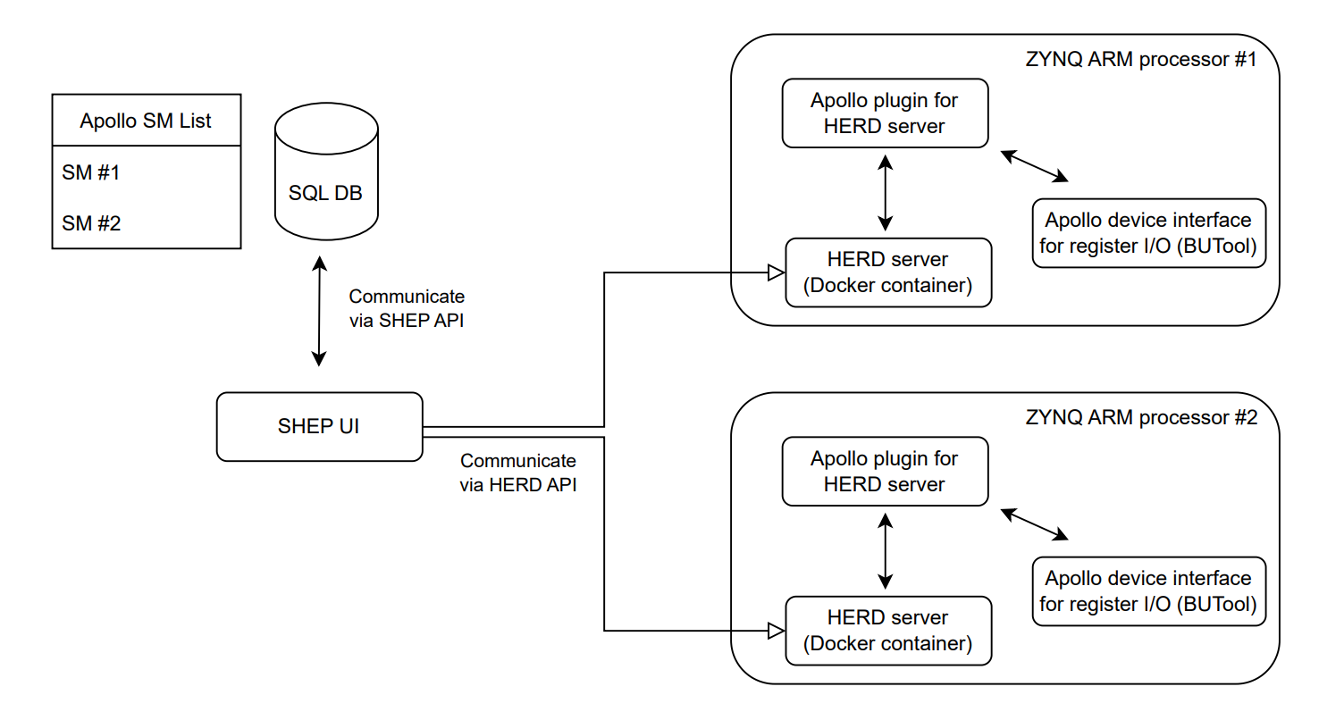
\includegraphics[width=0.9\textwidth]{TrackerUpgrade/SHEP_HERD.png}
    \caption{The schematic showing the communication between the SHEP UI and HERD API server, running on the Zynq SoC of each
    Apollo board. SHEP UI stores a list of boards in a SQL database, and communicates with each registered Apollo board by
    connecting to the HERD API server. The HERD application running on the SoC, in turn interfaces with Apollo-specific software
    to fulfill its tasks.}
    \label{fig:shep_herd_schematic}
\end{figure}

To make the deployment of the online software stack more standardized, SHEP and HERD software are currently designed to be run
as Docker containers that are communicating over the LAN. This way, every dependency of each piece of software is installed within
the Docker container, and the dependence on the underlying SoC platform is minimized. Continuous integration (CI) pipelines in
GitLab are developed such that Docker images for each software in the stack can be automatically built within the CI jobs, and
be stored in the GitLab container registry.

\clearpage
